%----------------------------------------------------------------------------------------
%	PACKAGES AND THEMES
%----------------------------------------------------------------------------------------
\documentclass[aspectratio=169,xcolor=dvipsnames]{beamer}
\usetheme{SimplePlus}
\setbeamertemplate{footline}[frame number]{}

\usepackage{hyperref}
\usepackage{graphicx} % Allows including images
\usepackage{booktabs} % Allows the use of \toprule, \midrule and \bottomrule in tables
\usepackage{siunitx}
\usepackage{import}
\usepackage{amsmath}
%\numberwithin{equation}{section}% numera eq come #section.#formula
\usepackage{amsthm}
\usepackage{stmaryrd}
\usepackage{amssymb}
\usepackage{wasysym}
\usepackage{cancel}
\usepackage{textcomp}
\usepackage{subcaption}
\definecolor{myred}{rgb}{0.545, 0.172, 0.031}
\usepackage{listings}
\definecolor{codegreen}{rgb}{0,0.6,0}
\definecolor{codegray}{rgb}{0.5,0.5,0.5}
\definecolor{codestring}{rgb}{0.623, 0.176, 0.588}
\definecolor{backcolour}{rgb}{0.96,0.96,0.96}
\definecolor{bbcolour}{rgb}{0.01,0.03,0.35}
\definecolor{indexcolour}{rgb}{0,0.4,0.4}
\definecolor{myOrange}{rgb}{0.933, 0.313, 0.066}
\definecolor{myBlue}{rgb}{0, 0.298, 0.8}
\lstdefinestyle{mystyle}{
	backgroundcolor=\color{backcolour},   
	commentstyle=\color{codegreen},
	classoffset=1,
	keywordstyle=\color{bbcolour},
	numberstyle=\tiny\color{codegray},
	stringstyle=\color{codestring},
	basicstyle=\ttfamily\small,
	breakatwhitespace=false,  
	breaklines=true,                 
	captionpos=b,                    
	keepspaces=false,                 
	numbers=left,                    
	numbersep=3pt,                  
	showspaces=false,                
	showstringspaces=false,
	showtabs=false,                  
	tabsize=2
}
\lstset{texcl=false, mathescape=true,style=mystyle}
\lstset{emph={%  
		i, j,X,n,Y,polarpattern,subfigure,pattern%
	},emphstyle={\color{bbcolour}}%
}%

%\usepackage{cleveref}
%----------------------------------------------------------------------------------------
%	TITLE PAGE
%----------------------------------------------------------------------------------------

\title[short title]{Deep learning e segmentazione per la biologia cellulare} % The short title appears at the bottom of every slide, the full title is only on the title page
\subtitle{Utilizzo del transfer learning in Matlab per l'identificazione di cellule in microscopia}

\author[Pin-Yen] {Alessandro Mastrofini}

\institute[NTU] % Your institution as it will appear on the bottom of every slide, may be shorthand to save space
{
Elaborazione di Immagini \\
Università degli Studi di Roma Tor Vergata% Your institution for the title page
}
\date{2022} % Date, can be changed to a custom date

\graphicspath{{figures/}} %Setting the graphicspat%h
\graphicspath{{figures/}} %Setting the graphicspath
\makeatletter
\providecommand*{\input@path}{}
\edef\input@path{{figures/}{}\input@path}% prepend
\makeatother



%----------------------------------------------------------------------------------------
%	PRESENTATION SLIDES
%----------------------------------------------------------------------------------------

\begin{document}

\begin{frame}
    % Print the title page as the first slide
    \titlepage
\end{frame}

%------------------------------------------------
\section{First Section}
%------------------------------------------------

\begin{frame}{Image segmentation}
	\begin{figure}
	\centering
\begin{minipage}{0.5\linewidth}
\begin{itemize}
	\item Pixel-based
	\item Edge-based
	\item Region-based
	\item Model-based
	\item \textbf{Supervised methods}
\end{itemize}
\vspace{0.1\linewidth}

\small{$\operatorname{CM}=\frac{T P}{T P+F N}=\frac{T P}{\text { Total arai in GT }}$}\\


\small{$
\operatorname{CR}=\frac{T P}{T P+F P}=\frac{T P}{\text { Total area in BW }}$}\\


\small{$
\operatorname{FM}=\frac{2 \cdot CM \cdot C R}{C M+C R} \in[0 ; 1]
$}

\end{minipage}
\begin{minipage}{0.35\linewidth}
\tiny{\def\svgwidth{\linewidth}
 \input{p.pdf_tex}}
\end{minipage}
\end{figure}
\end{frame}

\begin{frame}[fragile]{Transfer learning}

	\begin{figure}
\begin{minipage}{\linewidth}
	\tiny{\def\svgwidth{\linewidth}
		\input{CNN.pdf_tex}}
\end{minipage}
\vspace{0.03\linewidth}

\begin{minipage}{0.15\linewidth}
	\centering
 \texttt{\{B\}==1}\\
 \texttt{\{N\}==0}

\end{minipage}\hfill
\begin{minipage}{0.4\linewidth}
	\tiny{\begin{lstlisting}[language=Matlab,basicstyle=\tiny]
	pxds=pixelLabelDatastore(...
	strcat(newPath,'dataset\GT_TRAIN'),...
	["N","B"],[0 1]); 
		\end{lstlisting}}
\end{minipage}\hfill
\begin{minipage}{0.4\linewidth}
	\tiny{\begin{lstlisting}[language=Matlab,basicstyle=\tiny]
	pxLayer = pixelClassificationLayer(...
	'Name','labels','Classes',tbl.Name,...
	'ClassWeights',classWeights);
	\end{lstlisting}}
\end{minipage}\hfill
	\end{figure}

	
\end{frame}

\begin{frame}{Training dataset}
	

\begin{figure}
	\begin{minipage}{0.6\linewidth}
		\tiny{\def\svgwidth{\linewidth}
			\input{datastore.pdf_tex}}
	\end{minipage}\hspace{0.05\linewidth}
	\begin{minipage}{0.3\linewidth}
	\tiny{\def\svgwidth{\linewidth}
		\input{pximds.pdf_tex}}
\end{minipage}
\end{figure}
\begin{figure}
	\begin{minipage}{\linewidth}
	\tiny{\def\svgwidth{\linewidth}
		\input{diagram.pdf_tex}}
\end{minipage}
\end{figure}
\end{frame}

\begin{frame}[fragile]{Classification layer}
\begin{figure}
	\begin{minipage}{0.7\linewidth}
	\tiny{\begin{lstlisting}[language=Matlab,basicstyle=\tiny]
	lgraph = deeplabv3plusLayers(imageSize,numClasses,"resnet50"); 
	% balance predominance of 0
	tbl = countEachLabel(pximds);
	totalNumberOfPixels = sum(tbl.PixelCount);
	frequency = tbl.PixelCount / totalNumberOfPixels;
	classWeights = 1./frequency;
	pxLayer = pixelClassificationLayer('Name','labels','Classes',...
	tbl.Name,'ClassWeights',classWeights);
	lgraph = replaceLayer(lgraph,"classification",pxLayer);
	options = trainingOptions('sgdm','MaxEpochs',30, ...  
	'MiniBatchSize',8, 'Plots','training-progress');
	[net, info]= trainNetwork(pximds,lgraph,options);
\end{lstlisting}}
\centering
\vspace{5 mm}
\begin{minipage}{0.6\linewidth}
		\tiny{\def\svgwidth{\linewidth}
		\input{class.pdf_tex}}
\end{minipage}\hfill
\begin{minipage}{0.4\linewidth}
	\centering
	\fontsize{3}{4}\selectfont{$\begin{array}{cccccccccc}\text { B } & \text { B } & \text { B } & \text { B } & \text { B } & \text { B } & \text { B } & \text { B } & \text { B } \\ \text { B } & \text { B } & \text { B } & \text { B } & \text { B } & \text { B } & \text { B } & \text { B } & \text { B } \\ \text { B } & \text { B } & \text { B } & \text { B } & \text { B } & \text { B } & \text { B } & \text { B } & \text { B } \\ \text { N } & \text { B } & \text { B } & \text { B } & \text { B } & \text { B } & \text { B } & \text { B } & \text { B } \\ \text { N } & \text { B } & \text { B } & \text { B } & \text { B } & \text { B } & \text { B } & \text { B } & \text { B } \\ \text { N } & \text { N } & \text { B } & \text { B } & \text { B } & \text { B } & \text { B } & \text { B } & \text { B } \\ \text { N } & \text { N } & \text { N } & \text { B } & \text { B } & \text { B } & \text { B } & \text { B } & \text { B } \\ \text { N } & \text { N } & \text { N } & \text { N } & \text { B } & \text { B } & \text { B } & \text { B } & \text { B } \\ \text { N } & \text { N } & \text { N } & \text { N } & \text { N } & \text { B } & \text { B } & \text { B } & \text { B } \\ \text { N } & \text { N } & \text { N } & \text { N } & \text { N } & \text { N } & \text { B } & \text { B } & \text { B } \\ \text { N } & \text { N } & \text { N } & \text { N } & \text { N } & \text { N } & \text { N } & \text { N } & \text { N } \\ \text { N } & \text { N } & \text { N } & \text { N } & \text { N } & \text { N } & \text { N } & \text { N } & \text { N } \\ \text { N } & \text { N } & \text { N } & \text { N } & \text { N } & \text { N } & \text { N } & \text { N } & \text { N } \\ \text { N } & \text { N } & \text { N } & \text { N } & \text { N } & \text { N } & \text { N } & \text { N } & \text { N } \\ \text { N } & \text { N } & \text { N } & \text { N } & \text { N } & \text { N } & \text { N } & \text { N } & \text { N } \\ \text { N } & \text { N } & \text { N } & \text { N } & \text { N } & \text { N } & \text { N } & \text { N } & \text { N } \\ \text { N } & \text { N } & \text { N } & \text { N } & \text { N } & \text { N } & \text { N } & \text { N } & \text { N }\end{array}$}
\end{minipage}
	\end{minipage}\hfill
\begin{minipage}{0.3\linewidth}\centering
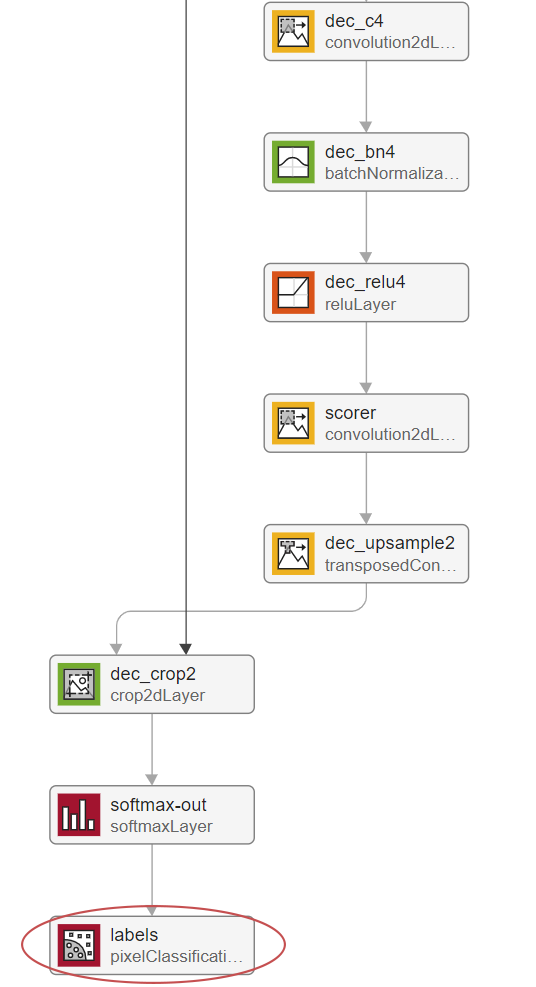
\includegraphics[width=0.9\linewidth]{lastlayers.png}
\end{minipage}
	
\end{figure}
\end{frame}

\begin{frame}{Training}
	\begin{figure}
		\begin{minipage}{0.8\linewidth}
			\centering
			\fontsize{3}{4}\selectfont{\def\svgwidth{\linewidth}
				\input{accuracy.pdf_tex}}\vspace{5 mm}
			\fontsize{3}{4}\selectfont{\def\svgwidth{\linewidth}
				\input{loss.pdf_tex}}
		\end{minipage}\hfill
		\begin{minipage}{0.2\linewidth}
\centering
\tiny{GPU consuming}
\vspace{5 mm}
\hspace{5 mm}\fontsize{3}{4}\selectfont{\def\svgwidth{0.9\linewidth}
	\input{gpu.pdf_tex}}
		\end{minipage}
		
	\end{figure}
\end{frame}

\begin{frame}[fragile]{Application}
	\begin{figure}
		\begin{minipage}{0.69\linewidth}
	\tiny{\begin{lstlisting}[language=Matlab,basicstyle=\tiny]
for l = 1:length(f_test)
	testImage=imread([strcat(dataPath,'/FRAME_TEST_SEG/'),f_test(l).name]);
	C_test = semanticseg(testImage,net);
	D=C_test=='B';
	GTImage=imread([strcat(dataPath,'/GT_TEST/'),gt_train(l).name]);
	[TP,FP,FN,CR,CM,FM_test(l)]=evaluation_segmentation(...
	bwareafilt(D,1),GTImage);
	imshowpair(testImage,bwareafilt(D,1),'montage');
	pause(0.5); drawnow;
	clear C_test D testImage;
end
\end{lstlisting}}
		\end{minipage}\hfill
	\begin{minipage}{0.3\linewidth}
			\fontsize{3}{4}\selectfont{\def\svgwidth{0.8\linewidth}
			\input{FM_first.pdf_tex}}
	\end{minipage}
\centering
\tiny{n. 25:}\\
\begin{minipage}{0.25\linewidth}
	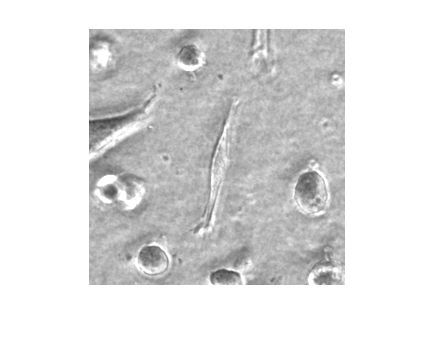
\includegraphics[width=\linewidth]{n25.png}
\end{minipage}\hfill
\begin{minipage}{0.25\linewidth}
	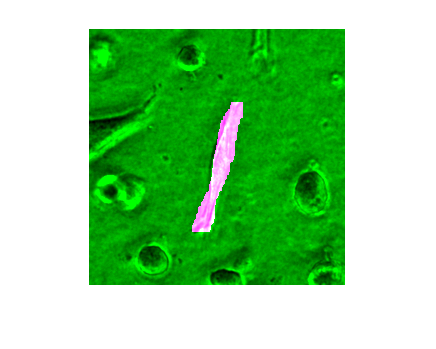
\includegraphics[width=\linewidth]{n25_GT.png}
\end{minipage}\hfill
\begin{minipage}{0.25\linewidth}
	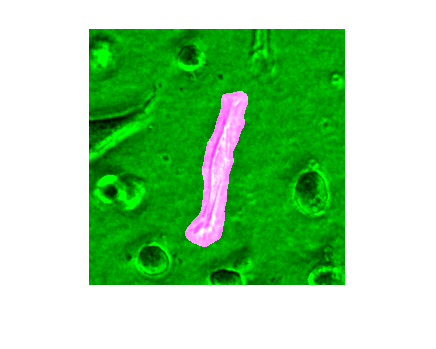
\includegraphics[width=\linewidth]{n25_seg.png}
\end{minipage}\hfill
\begin{minipage}{0.25\linewidth}
	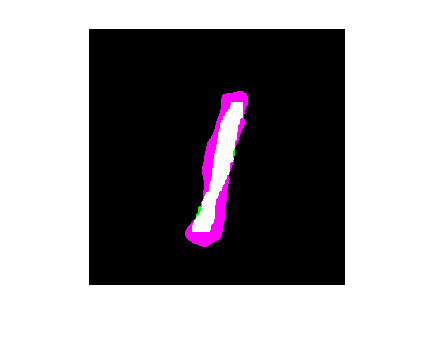
\includegraphics[width=\linewidth]{GT_vs_SEG.png}
\end{minipage}\hfill
	\end{figure}
\end{frame}

\begin{frame}{Solver}
\begin{figure}
	\centering
	\begin{minipage}{\linewidth}
		\centering
		\fontsize{3}{4}\selectfont{\def\svgwidth{0.9\linewidth}
			\input{solver.pdf_tex}}
	\end{minipage}
\end{figure}	
	
\end{frame}

\begin{frame}{Training options}
\begin{figure}
	\centering
	\begin{minipage}{0.3\linewidth}
		\centering
		\footnotesize{numbers of epochs}\\\vspace{2 mm}
		\fontsize{3}{4}\selectfont{\def\svgwidth{0.9\linewidth}
			\input{epoche.pdf_tex}}\vspace{1 mm}
			\fontsize{3}{4}\selectfont{\def\svgwidth{0.9\linewidth}
			\input{epoche2.pdf_tex}}
	\end{minipage}
	\begin{minipage}{0.3\linewidth}
	\centering
	\footnotesize{mini batch size}\\\vspace{2 mm}
	\fontsize{3}{4}\selectfont{\def\svgwidth{0.9\linewidth}
		\input{batch.pdf_tex}}\vspace{1 mm}
	\fontsize{3}{4}\selectfont{\def\svgwidth{0.9\linewidth}
		\input{batch2.pdf_tex}}
\end{minipage}
	\begin{minipage}{0.3\linewidth}
	\centering
	\footnotesize{numbers of epochs}\\\vspace{2 mm}
	\fontsize{3}{4}\selectfont{\def\svgwidth{0.9\linewidth}
		\input{lr.pdf_tex}}\vspace{1 mm}
	\fontsize{3}{4}\selectfont{\def\svgwidth{0.9\linewidth}
		\input{lr2.pdf_tex}}
\end{minipage}
\end{figure}	
\end{frame}

\begin{frame}{Augmenter}
	\begin{figure}
		\centering
		\begin{minipage}{0.5\linewidth}
			\centering
		\tiny{only rotation\\ \texttt{mean}: 0.4659}
		\end{minipage}\hfill
		\begin{minipage}{0.5\linewidth}
			\centering
			\tiny{only reflection\\ \texttt{mean}: 0.7989}
		\end{minipage}\hfill
		\begin{minipage}{0.5\linewidth}
			\vspace{5 mm}
			\centering
			\tiny{only traslation}
				\fontsize{3}{4}\selectfont{\def\svgwidth{0.9\linewidth}
				\input{contour1.pdf_tex}}
		\end{minipage}\hfill
		\begin{minipage}{0.5\linewidth}
		\centering
		\vspace{5 mm}
		\tiny{all}\\
		\fontsize{3}{4}\selectfont{\def\svgwidth{0.9\linewidth}
			\input{contour2.pdf_tex}}
	\end{minipage}
	\end{figure}	
\end{frame}


\begin{frame}[fragile]{Pretrained networks}
	
	\begin{figure}
		\centering\hspace{5 mm}
\begin{minipage}{0.2\linewidth}\centering
	\tiny{\def\svgwidth{\linewidth}
	\input{moreNet.pdf_tex}}
\end{minipage}\hfill
\begin{minipage}{0.7\linewidth}
	\centering
	\tiny{\def\svgwidth{0.85\linewidth}
	\input{net.pdf_tex}}
\end{minipage}
	\begin{minipage}{0.9\linewidth}
	\tiny{\begin{lstlisting}[language=Matlab,basicstyle=\tiny]
	clear pximds lgraph
	[pximds,lgraph]=prepareMyNet(net,'netName',imds,pxds);
	[net_net,info_net,FM_test_net,compTime_net]=trainAndTest(pximds,lgraph,...
	dataPath,f_test,gt_train);	
	[accuracy_net,loss_net,FM_mean_net]=figureAccAndLoss(info_net,FM_test_net)
	\end{lstlisting}}
\end{minipage}
	\end{figure}
\end{frame}

\begin{frame}[fragile]{Border identification}
\begin{figure}
	\begin{minipage}{0.6\linewidth}
	\fontsize{3}{4}\selectfont{\def\svgwidth{0.95\linewidth}
	\input{mole.pdf_tex}}
	\end{minipage}\hfill
\begin{minipage}{0.4\linewidth}
		\fontsize{5}{4}\selectfont{$\begin{array}{ccccc}
			\text { INSIDE } & \text { INSIDE } & \text { BORDER } & \text { BORDER } & \text { BACK } \\ \text { INSIDE } & \text { INSIDE } & \text { BORDER } & \text { BORDER } & \text { BACK } \\ \text { INSIDE } & \text { INSIDE } & \text { BORDER } & \text { BORDER } & \text { BACK } \\ \text { INSIDE } & \text { INSIDE } & \text { BORDER } & \text { BORDER } & \text { BACK } \\ \text { INSIDE } & \text { INSIDE } & \text { BORDER } & \text { BORDER } & \text { BACK } \\ \text { INSIDE } & \text { INSIDE } & \text { BORDER } & \text { BORDER } & \text { BACK } \\ \text { INSIDE } & \text { INSIDE } & \text { BORDER } & \text { BORDER } & \text { BACK } \\ \text { INSIDE } & \text { INSIDE } & \text { BORDER } & \text { BORDER } & \text { BACK } \\ \text { INSIDE } & \text { INSIDE } & \text { BORDER } & \text { BORDER } & \text { BACK } \\ \text { INSIDE } & \text { INSIDE } & \text { BORDER } & \text { BORDER } & \text { BACK } \\ \text { INSIDE } & \text { INSIDE } & \text { BORDER } & \text { BORDER } & \text { BACK } \\ \text { INSIDE } & \text { INSIDE } & \text { BORDER } & \text { BORDER } & \text { BACK } \\ \text { INSIDE } & \text { INSIDE } & \text { BORDER } & \text { BORDER } & \text { BACK }\end{array}$}
\end{minipage}
\begin{minipage}{\linewidth}
		\tiny{\begin{lstlisting}[language=Matlab,basicstyle=\tiny]
	pathImage = strcat(newPath,'dataset\mole\Immagini');
	pathGT=strcat(newPath,'dataset\mole\Segmentazioni');
	pathExport=strcat(newPath,'dataset\mole\PROCESSED\');
	[imds,pxds]=optimizeDataset(pathImage,pathGT,pathExport,8,imageSize);
	%
	imdsTEST = imageDatastore(strcat(newPath,'dataset\mole\TEST\Immagini')); 
	\end{lstlisting}}
\end{minipage}\hfill
\begin{minipage}{0.1\linewidth}
	\centering

\includegraphics[width=\linewidth]{element.pdf}
\end{minipage}\hfill
\begin{minipage}{0.2\linewidth}
	\centering
	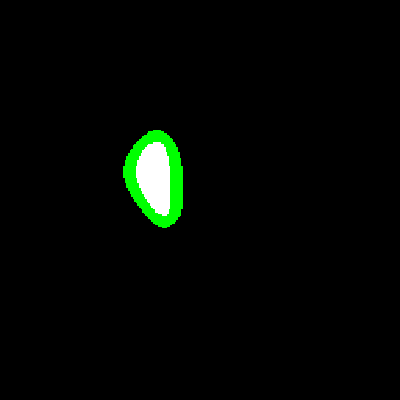
\includegraphics[width=0.9\linewidth]{eroded.pdf}
\end{minipage}\hfill
\begin{minipage}{0.55\linewidth}
	\tiny{\begin{lstlisting}[language=Matlab,basicstyle=\tiny]
	temp_GT=imread(string(startingGT.Files(i)));
	temp_INT=imerode(temp_GT,SE);
	temp_INT=imbinarize(temp_INT); 
	temp_GT=imbinarize(temp_GT);
	temp_GT=uint8(temp_GT);
	temp_INT=uint8(temp_INT);
	imshowpair(255*temp_GT,255*temp_INT)
	GT=temp_GT+temp_INT;
	GT=imresize(GT,imageSize(1:2));
	pathSplit=strsplit(string(startingGT.Files(i)),'\');
	imwrite(GT,strcat(pathExport,'GT\',pathSplit(end)))
\end{lstlisting}}
\end{minipage}
\end{figure}
\end{frame}

\begin{frame}[fragile]{Training}
	\begin{figure}
		\begin{minipage}{0.42\linewidth}
				\fontsize{3}{4}\selectfont{\def\svgwidth{\linewidth}
				\input{acc.pdf_tex}}
				\fontsize{3}{4}\selectfont{\def\svgwidth{0.99\linewidth}
				\input{lox.pdf_tex}}
		\end{minipage}\hfill
	\begin{minipage}{0.53\linewidth}
	\tiny{\begin{lstlisting}[language=Matlab,basicstyle=\tiny]
	dsTrain = transform(dsTrain,...
	@(data)augmentImageAndLabel(data,xT,yT));
	\end{lstlisting}}
	\tiny{\begin{lstlisting}[language=Matlab,basicstyle=\tiny]
	function data = augmentImageAndLabel(data,xT,yT)
	for i = 1:size(data,1)
	tform = randomAffine2d('Rotation',[0 360],...
	'XReflection',true,'XTranslation', xTrans, ...
	'YTranslation', yTrans);
	rout = affineOutputView(size(data{i,1}), tform,...
	'BoundsStyle','centerOutput');
	data{i,1} = imwarp(data{i,1},tform,'OutputView',rout);
	data{i,2} = imwarp(data{i,2},tform,'OutputView',rout);
	end
	end	
\end{lstlisting}}
	\tiny{\begin{lstlisting}[language=Matlab,basicstyle=\tiny]
	[net, info]= trainNetwork(dsTrain,lgraph,options);
\end{lstlisting}}
\end{minipage}
	\end{figure}
\end{frame}

\begin{frame}{Segmentation}
	\begin{figure}
		\begin{minipage}{\linewidth}
			\centering

\includegraphics[width=0.2\linewidth]{inside.pdf}\hspace{0.08\linewidth}

\includegraphics[width=0.2\linewidth]{border.pdf}\hspace{0.08\linewidth}

\includegraphics[width=0.2\linewidth]{back.pdf}
		\end{minipage}\hfill
	\vspace{5 mm}
\begin{minipage}{0.25\linewidth}
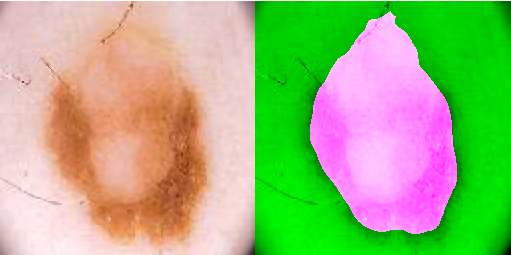
\includegraphics[width=\linewidth]{11.png}\vspace{2 mm}
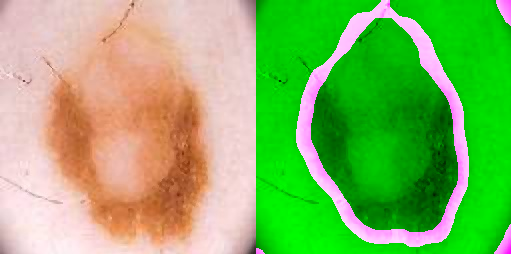
\includegraphics[width=\linewidth]{12.png}
\end{minipage}\hspace{0.05\linewidth}
\begin{minipage}{0.25\linewidth}
	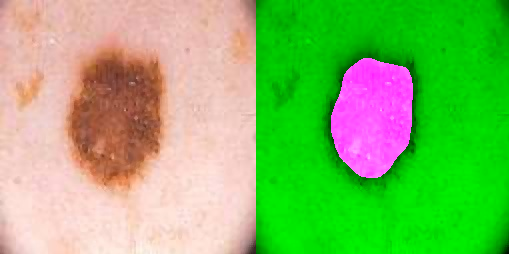
\includegraphics[width=\linewidth]{41.png}\vspace{2 mm}
	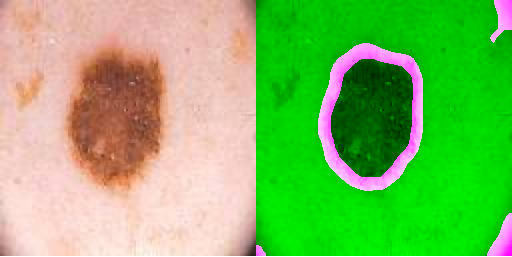
\includegraphics[width=\linewidth]{42.png}
\end{minipage}\hspace{0.05\linewidth}
\begin{minipage}{0.25\linewidth}
	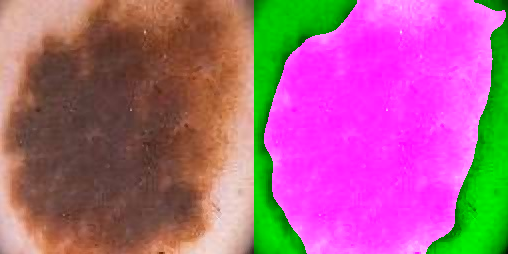
\includegraphics[width=\linewidth]{281.png}\vspace{2 mm}
	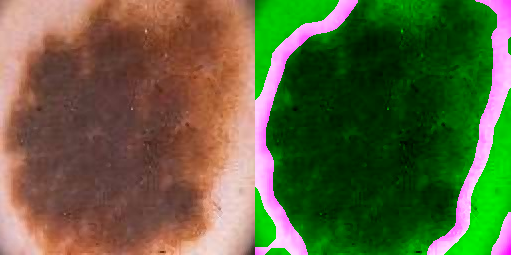
\includegraphics[width=\linewidth]{282.png}
\end{minipage}

	\end{figure}
\end{frame}

\end{document}